\documentclass{article}

\usepackage{amsmath,amssymb,amsthm}
\usepackage{float}
\usepackage{amsmath,amssymb,amsthm}
\usepackage{graphicx}
\setlength{\oddsidemargin}{0.25 in}
\setlength{\evensidemargin}{-0.25 in}
\setlength{\topmargin}{-0.6 in}
\setlength{\textwidth}{6.5 in}
\setlength{\textheight}{8.5 in}
\setlength{\headsep}{0.75 in}
\setlength{\parindent}{0 in}
\setlength{\parskip}{0.1 in}

\newtheorem{theorem}{Theorem}
\newtheorem{corollary}{Corollary}
\newtheorem{proposition}{Proposition}
\newtheorem*{remark}{Remark}
\theoremstyle{definition}
\newtheorem{example}{Example}
\newtheorem{definition}{Definition}

\newcommand{\lecture}[4]{
   \pagestyle{myheadings}
   \thispagestyle{plain}
   \newpage
%   \setcounter{lecnum}{#1}
   \setcounter{page}{1}
   \noindent
   \begin{center}
   \framebox{
      \vbox{\vspace{2mm}
    \hbox to 6.58in { {\bf CSC~565: Graph Theory
                        \hfill North Carolina State University} }
    \hbox to 6.58in { {\bf Fall 2019
                        \hfill Computer Science} }
       \vspace{4mm}
       \hbox to 6.28in { {\Large \hfill Lecture #1: #2  \hfill} }
       \vspace{2mm}
       \hbox to 6.28in { {\it Lecturer: {\it Don Sheehy {\tt <drsheehy@ncsu.edu>}} \hfill Scribe: #4} }
      \vspace{2mm}}
   }
   \end{center}
   \markboth{Lecture #1: #2}{Lecture #1: #2}
   \vspace*{4mm}
}

\usepackage{changepage}
\begin{document}

  \title{Lecture 22}
  \author{Scribed by: Ellis Ackerman and Roshani Narasimhan}
  \date{November 6, 2019}
  \maketitle
  
  \noindent \textbf{Proving Steinitz's Theorem}
  \newline \noindent With the addition of an additional lemma, we will have the tools to formalize a constructive proof for \textit{Steinitz's Theorem}. (Recall that Steinitz's theorem states that a graph is polytopal iff it is planar and three-connected.)
  
  \medskip \noindent We will follow the following steps to prove the theorem:
  \begin{itemize}
      \item Use Tutte's algorithm to find a linear embedding of the graph.
      \item Lift the faces using the Maxwell correspondence.
  \end{itemize}
  \medskip  \noindent \textbf{Lemma:} Let $G$ be a planar and 3-connected graph, then either $G$ has $K_3$ has a non-separating induced cycle, or the dual, $G^*$ has a $K_3$ as a non-separating induced cycle. 
  
  \medskip \noindent Points to note:
  \begin{itemize}
      \item $K_3$ is the smallest induced cycle that is possible.
      \item The dual of a polygon will also be a polygon. In general, the dual of an n-gon will be an n-gon.
  \end{itemize}
  \smallskip  \noindent \textit{Proof.} For the sake of a contradiction suppose that both $G=(V,E)$ and its dual, $G^*=(V^*,E^*)$ have no triangle faces. Let $n=|V_G|$, $m=|E_G|$ and $f$ be the number of faces in the embedding of $G$. Then by Euler's Formula, $n-m+f=2$, but since we have no triangular faces, every face is bounded by more than three edges. Thus, $2m \geq 4f$ so $m \geq 2f$. Thus, $2=n-m+f \leq n -2f +f = n-f$. Now consider $G^*$. We see that $m \geq 2n$ (since the number of faces and vertices switches in the dual). This leads us to the conclusion $2=n-m+f \leq n-2n+f=f-n$. Notice, $2=n-f$ and $2=f-n$. We have reached our contradiction. Thus, for a planar and 3-connected graph $G$, either $G$ or $G^*$ has a triangular face. 
 \vspace{0.5mm} \begin{flushright} $\square$ \end{flushright}
  
 \medskip \noindent We are now positioned to prove Steinitz's Theorem.
  
  \begin{theorem}
    $G$ is polytopal if and only if $G$ is planar and 3-connected.
  \end{theorem}
  \begin{proof}
    Let $G$ be a planar and 3-connected graph. 
    \smallskip \newline \noindent \textit{Case 1:} Additionally, suppose that $G$ has some face which is $K_3$. Let us embed the graph, via Tutte's Algorithm such that the $K_3$ face is the outer face. We now lift the embedding from the plane using the Maxwell Correspondence, for everything but the outer face. We now have an an unbounded polyhedron. We now lift the outer-face up, and since in three dimensional space, three points form a flat surface. The outer-face from $G$ becomes the bounding upper face of the polyhedron, and we now have that $G$ is indeed a polytope.
    \smallskip \newline \noindent \textit{Case 2:} Suppose that $G$ has no $K_3$ face. Then by the Lemma, we know that $G^*$ has a $K_3$ face. We no proceed to \textit{case 1} and now have a polytope, call it $P^*$, for $G^*$. We know that for some polytope, there is a polar-polytope whose graph is its dual. Thus, for $P^*$, there is a polytope, $P$, whose graph is $(G^*)^* = G$. 
    \newline \noindent The other direction has already been proved, thus we are done. 
  \end{proof}

 \bigskip \noindent \textbf{Algebraic Graph Theory}
 \newline \noindent To better understand the geometric realizations of graphs, as discussed earlier, and graph morphisms between these realizations, we turn out attention to the algebraic elements of graph theory. 
 \smallskip \newline \noindent \textbf{Definition:} A \textit{vector space} is a set $V$ and a field $F$ with and addition operation between set elements and scalar multiplication between field and set elements. Formally, the following conditions must be satisfied: 
 \begin{adjustwidth}{2.5em}{0pt}
 1. $u+v=v+u$ for all $u,v \in V$ (addition commutes).
 \newline 2. $s(u+v)=su+sv$ for all $u,v \in V$ and $s \in F$ (scalar multiplication distributes).
 \newline 3. $w+(u+v)=(w+u)+v$ for all $u,v,w \in V$ (addition is associative).
 \newline There exists a unique zero vector, \textbf{0} such that $v+\text{\textbf{0}}=\text{\textbf{0}}+v=v$ for all $v \in V$.
 \newline \noindent 4. There exists a unique additive inverse such that $v+v' = v'+v=\text{\textbf{0}}$ for all $v \in V$, usually we denote the additive inverse for $v$ by $-v$.
\end{adjustwidth}

Examples of vector spaces include the set of continuous functions and the set of polynomials.

\medskip \noindent Now consider a function, $f$, between vector spaces. Let $V$ be a finite dimensional vector space over a field $F$ and $U$ be a finite dimensional vector space over the same field. 
\newline \noindent \textbf{Definition:} The function $f: V \rightarrow U$ is said to be a \textit{linear} if: 
\begin{adjustwidth}{2.5em}{0pt}
1. $f(u+v)=f(u)+f(v)$ for all $u,v \in V$.
\newline \noindent 2. $f(kv) = kf(v)$ for all $v \in V$ and $k \in F$.
\end{adjustwidth}

\medskip \noindent \textbf{Matrices as maps from one vector space to another:}
Let us consider matrices to convert a vector in one vector space to a vector in another vector space. Let $x$ be the vector in the $U$ and $b$ be the vector in the vector space $V$. The matrix $A$ will map the vector $x$ in $U$ to the vector $b$ in $V$ by $Ax=b$. To solve $Ax=b$, we multiply by $A^{-1}$ so that $A^{-1}Ax=A^{-1}b$ and $x=A^{-1}b$. This is essentially transforming $b$ into $x$, we are trying to invert a linear operation. Note that if we have multiple solutions to map $x$ to $b$, then $A^{-1}$ won't exist (as solution is not unique), but solutions do exist.

\medskip \noindent \textbf{Definition:} The \textit{Adjacency Matrix} is the a matrix representation of connectivity in a graph. Consider a graph, $G=(V,E)$ where $n=|V|$. Then the adjacency matrix of $G$ is the matrix, $$A_G = (a_{ij})_{n \times n} = \begin{cases} 
      1 & \text{if } (v_i,v_j) \in E \\
      0 & \text{otherwise} \\
   \end{cases}
.$$
\noindent Note that the adjacency matrix is an inefficient data structure to store the graph information. This is because we observe that $A_G$ is symmetric for any graph $G$. Thus the information we actually need is stored twice. Most real world graphs are sparse and thus the adjacency matrix will  predominately contain zeros. (More zeros than ones).
\smallskip \newline \noindent \textit{Is the adjacency matrix a graph invariant?} Consider the graph, $G$, below and an isomorphic graph, $H$, obtained by permuting the vertices of $G$. 

\noindent 
\begin{figure}[H]
\centering
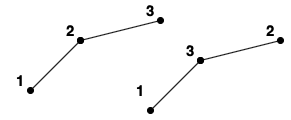
\includegraphics[scale=0.5]{Images/isomorphic_graphs.png}
\caption{Comparing the adjacency matrices for isomorphic graphs}
\label{fig:my_label}
\end{figure}  

\noindent Clearly, the graphs will not have the same adjacency matrices, since $$A_G = \bmat{0&1&0\\1&0&1\\0&1&0} \neq \bmat{0&0&1\\0&0&1\\1&1&0} = A_H.$$ But if there is a permutation matrix, such that $A_G = P^{-1}A_HP$, then $A_G$ and $A_H$ are said to be similar matrices. In this case, the desired permutation matrix is $$P=\bmat{1&0&0\\0&0&1\\0&1&0}.$$ While the adjacency matrix is not invariant in the stronger sense, it is invariant across the similarity of matrices. This is not very helpful in practice since finding the permutation matrix is computationally the same as finding an isomorphism between the graphs. Later, we will see an algebraic invariant that we will be able to directly compute, without having to worry about similarity or computing an intermediate step. 

\end{document}
